\section{Results}

\subsection{NLM agreement processing in Italian}
\paragraph{Ablation results}
\paragraph{Dynamics of the number unit} in nounpp, pointing (again) to Fig.~\ref{fig:nounpp}.

\begin{figure}
    \centering
    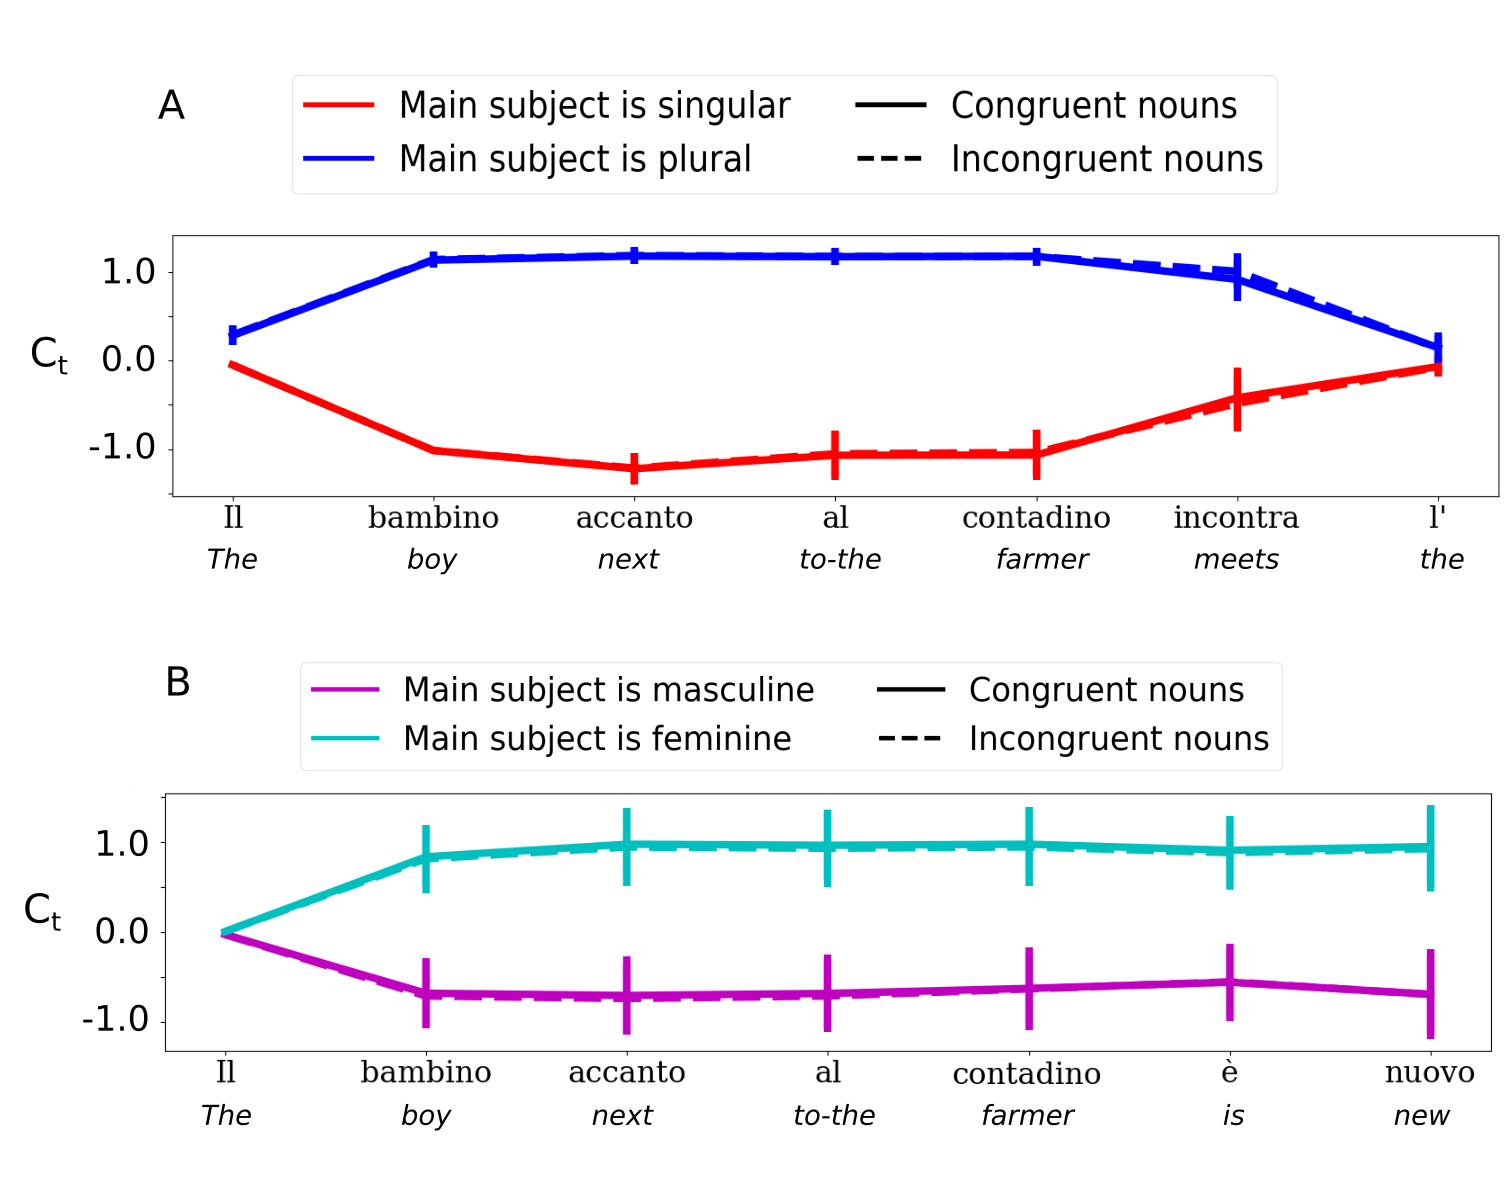
\includegraphics[width=\textwidth]{figures/model_activations_nounpp.png}
    \caption{\textbf{Cell activity of the number unit (panel A) and gender unit (panel B) during the processing of a single long-range dependency across a prepositional phrase:} four conditions are presented, corresponding to whether the main subject of the sentence is singular (red curves) or plural (blue), and to whether the main subject (`bambino') and the intervening noun (`contadino') have the same (congruent) or opposite number (incongruent)}
    \label{fig:nounpp}
\end{figure} 


\subsection{Nested Dependencies in NLMs and Subjects}

\paragraph{Dynamics of the number unit in NLM processing of nested dependencies}

\begin{itemize}
\item We confirm the behaviour we expect, as exemplified in \ref{fig:nested_dynamics}.
\end{itemize}

\begin{figure*}
    \centering
    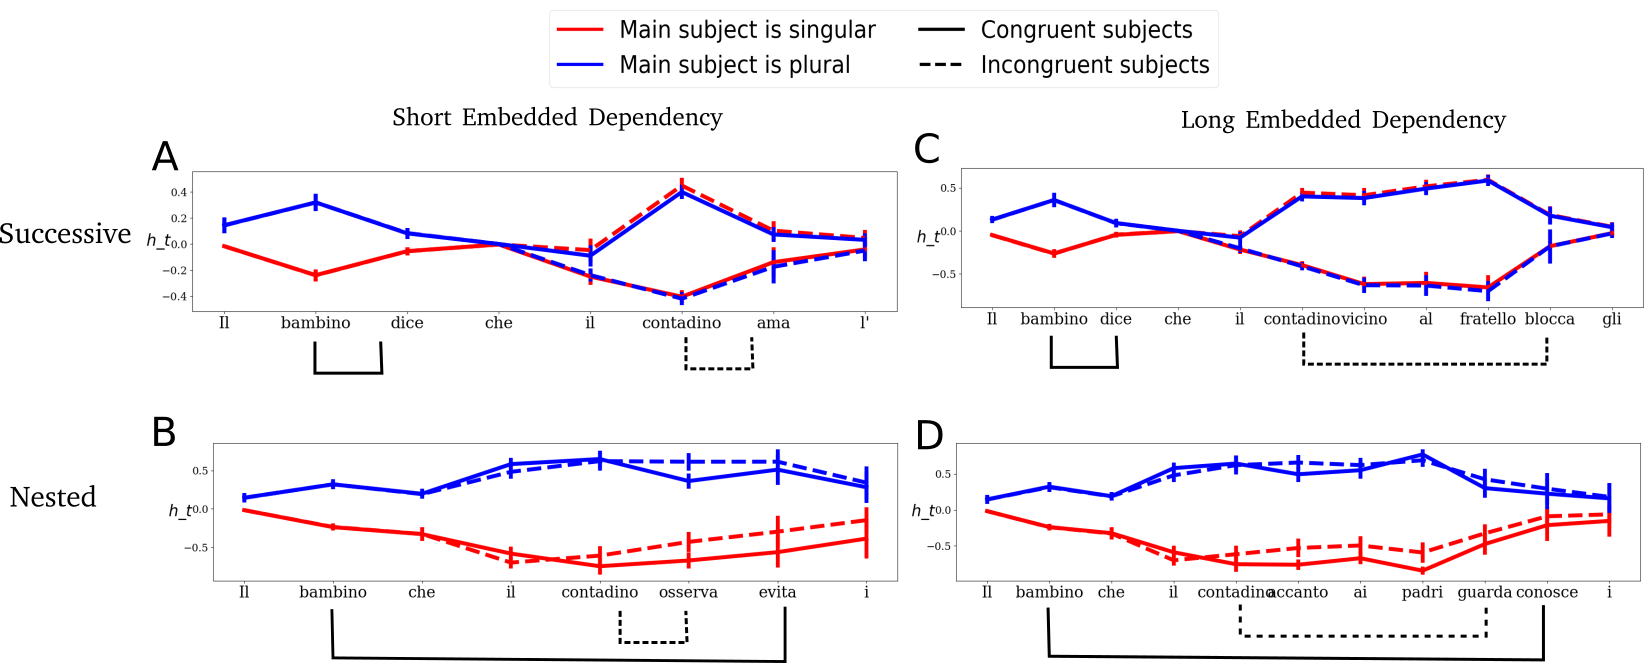
\includegraphics[width=\textwidth]{figures/model_activations.png}
    \caption{\textbf{Dynamics of the hidden activation of the number unit during the processing of two subject-verb dependencies.} Number-unit activity is presented for the four structures in the design: SC-short (panel A), SC-long (B), objRC-short (C) and objRC-long (D). For each structure, results are presented for the four conditions, corresponding to whether the main subject of the sentence is singular (red curves) or plural (blue), and to whether the main and embedded subjects have the same grammatical number (congruent; continuous lines) or not (incongruent; dashed lines).}
    \label{fig:nested_dynamics}
\end{figure*}

\paragraph{Comparing NLM and subject performance}

\begin{itemize}
\item Discuss figures \ref{fig:SC_results} and \ref{fig:objRC_results},
\end{itemize}

\begin{figure*}[h]
    \centering
    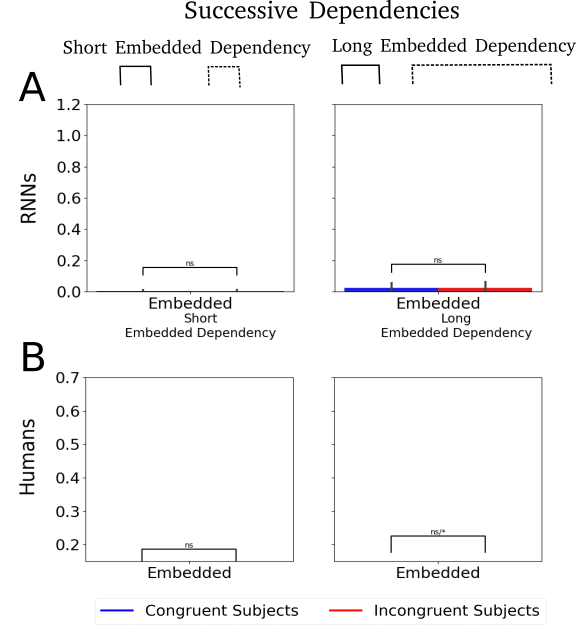
\includegraphics[width=10cm]{figures/error_rates_successive.png}
    \caption{\textbf{Error rates on the SC-short and SC-long structures:} collected from NLMs (panel A) and human subjects (B). Blue and red bars correspond to whether the main and embedded subjects agree on number (congruent subjects) or not (incongruent), respectively). Error bars represent standard error of the mean across all trials. ns - non significant.}
    \label{fig:SC_results}
\end{figure*}


\begin{figure*}[h]
    \centering
    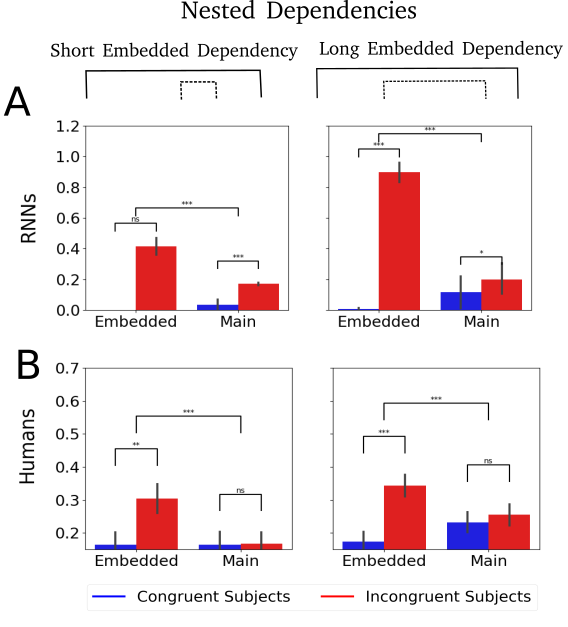
\includegraphics[width=10cm]{figures/error_rates_nested.png}
    \caption{\textbf{Error rates on the objRC-short and objRC-long structures:} collected from NLMs (panel A) and humans subjects (panel B). Blue and red bars correspond to whether the main and embedded subjects agree on number (congruent subjects) or not (incongruent), respectively. Error bars represent standard error of the mean across all trials. ns - non significant.}
    \label{fig:objRC_results}
\end{figure*}

% \lipsum[1]
